\documentclass{article}

% Margins.
\setlength{\oddsidemargin}{0in}
\setlength{\evensidemargin}{0in}
\setlength{\headheight}{12pt}
\setlength{\headsep}{42pt}
\setlength{\topmargin}{-54pt}
\setlength{\textwidth}{6.5in}
\setlength{\textheight}{9in}

\usepackage{float}
\usepackage{graphicx}

%opening
\title{Programming for Engineers I\\Creating a New Project in Visual Studio}
\author{Attique Dawood}

\begin{document}

\maketitle

\section{Solution and Projects}
In Visual Studio 2003--2010 a \emph{project} must be created before the code can be compiled into an executable (exe). A project will produce exactly one exe therefore every project must contain at least one code/.cpp file and a \verb|main()| function. Projects are contained in something called a \emph{solution}. A solution may contain more than one projects. Projects \emph{must} be part of a solution even if there is only one project in a solution. Projects or code/.cpp files cannot be compiled separately.

\section{Creating a New Solution and Project}
\subsection{New Project Dialog}
In Visual Studio navigate to \verb|File > New > Project|. A dialog box containing additional options will appear.
\begin{figure}[H]
\centering
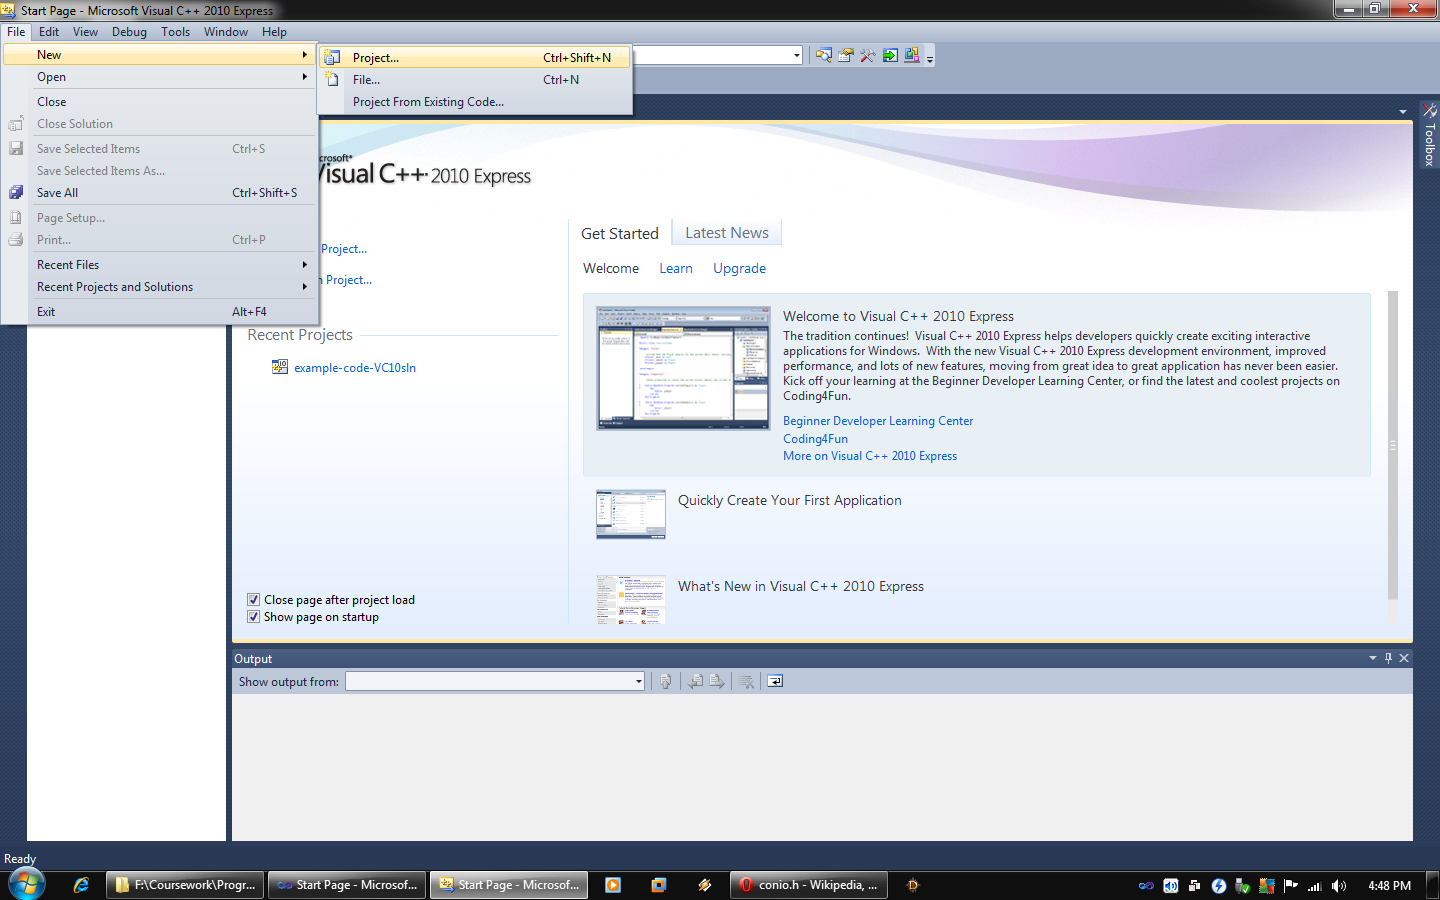
\includegraphics[width=\textwidth]{Create_New_Project.png}
\caption{Creating a new project and solution}
\end{figure}
\begin{figure}[H]
\centering
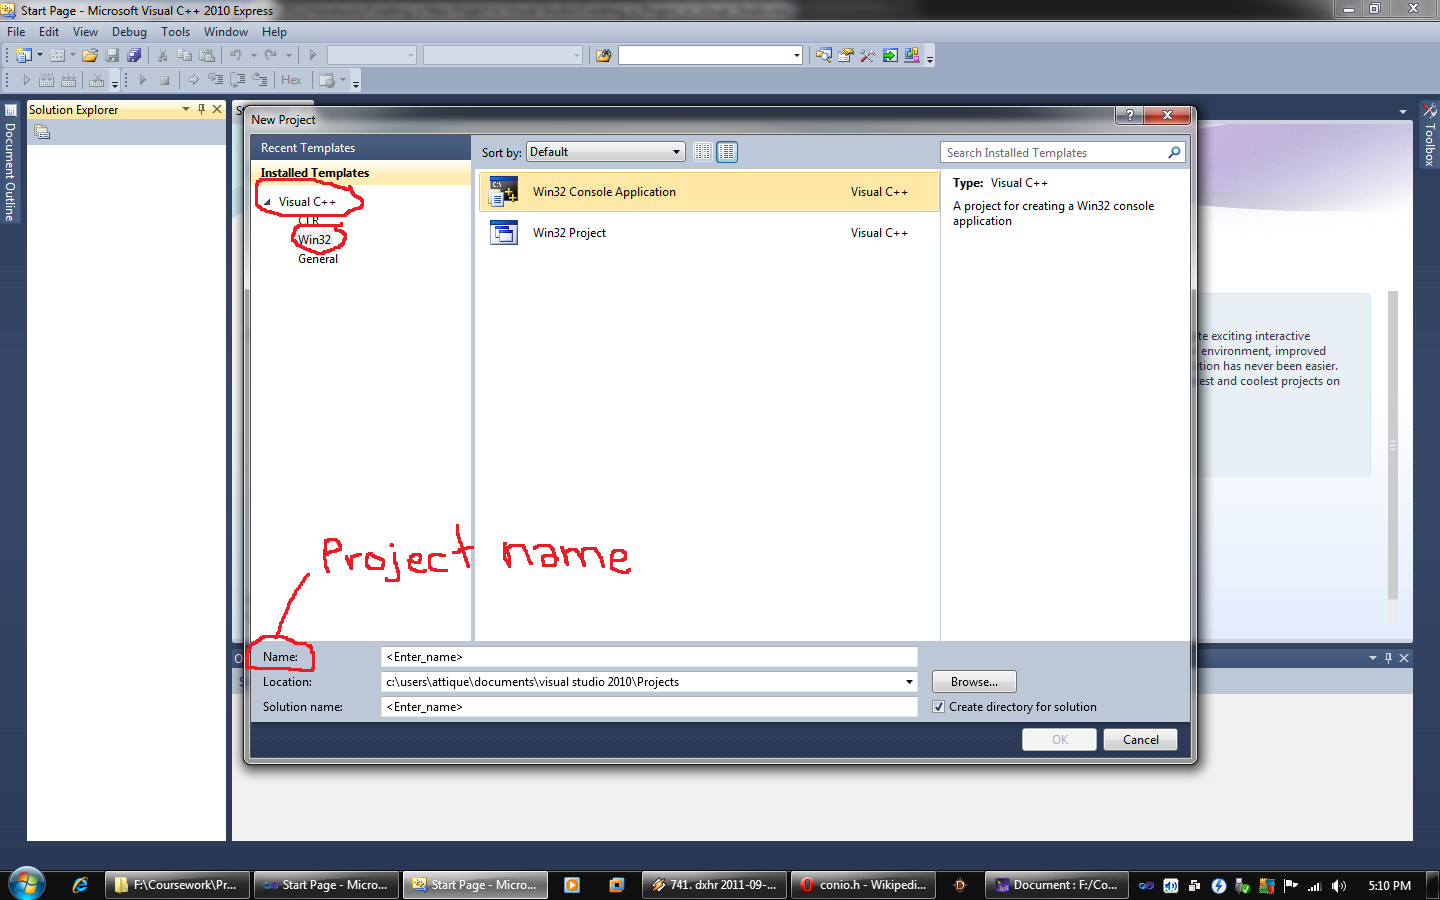
\includegraphics[width=\textwidth]{New_Project_Dialog.png}
\caption{New Project Dialog Box}
\end{figure}
Make sure you select \verb|Visual C++ > Win32| from the template options on the left and\\ \verb|Win32 Console Application| from the additional list of projects.

\subsection{Naming Your Solution and Project}
Most assignments require you to submit multiple programs or code/.cpp files for each exercise or question. It is a good idea to create a single solution for assignment. For each exercise or question in an assignment you can create a separate project. You have the option to build (or compile) projects in a solution at once. Also, when you open a solution file (.sln) all projects within that solution will be visible and can be managed.

For this example, we will assume that we are required to submit three programs (or exercises) from Assignment No. 2. We will name our project as \verb|Question No 1| and the solution will be called \verb|Assignment 2|. Notice the location or path for the solution. Your solutions are by default created in the \verb|My Documents| folder.
\begin{figure}[H]
\centering
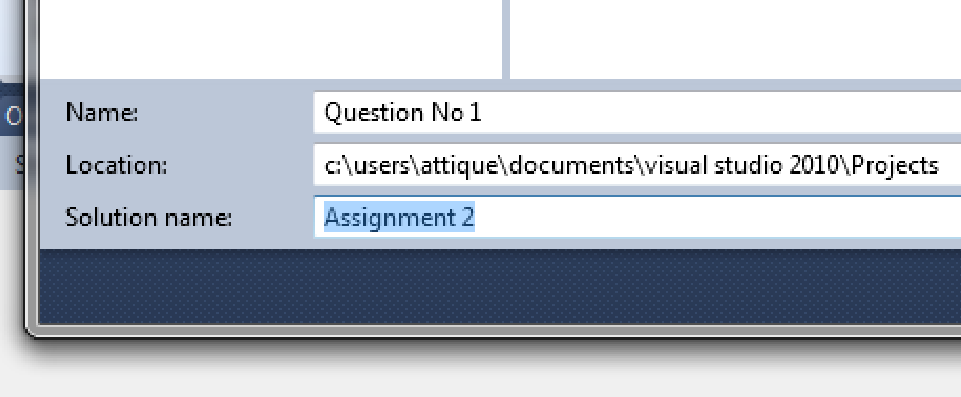
\includegraphics[width=\textwidth]{Naming_Solution_Project.png}
\caption{Project name, solution name and path/location}
\end{figure}
\subsection{Application Settings}
Click \verb|OK| and \verb|Win32 Application Wizard| will open. From here you \emph{\bfseries must} check \verb|Empty Project| before proceeding. In the \verb|Application Type| make sure \verb|Console Application| is checked. Click \verb|Finish| and your solution will be created.
\begin{figure}[h]
\centering
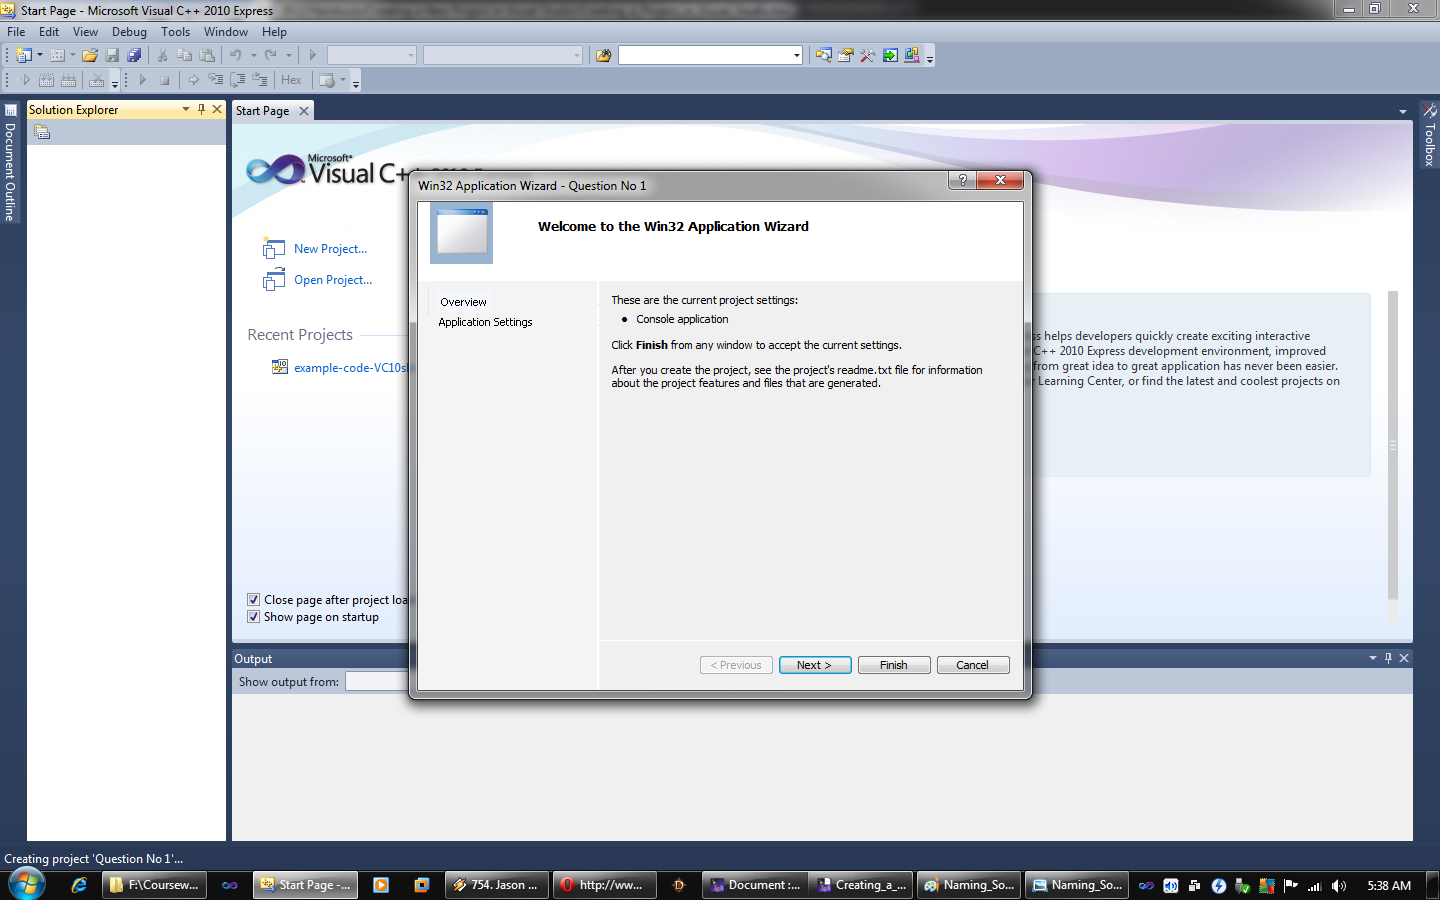
\includegraphics[width=\textwidth]{Win32_Application_Wizard.png}
\caption{Win32 Application Wizard}
\end{figure}
\begin{figure}[H]
\centering
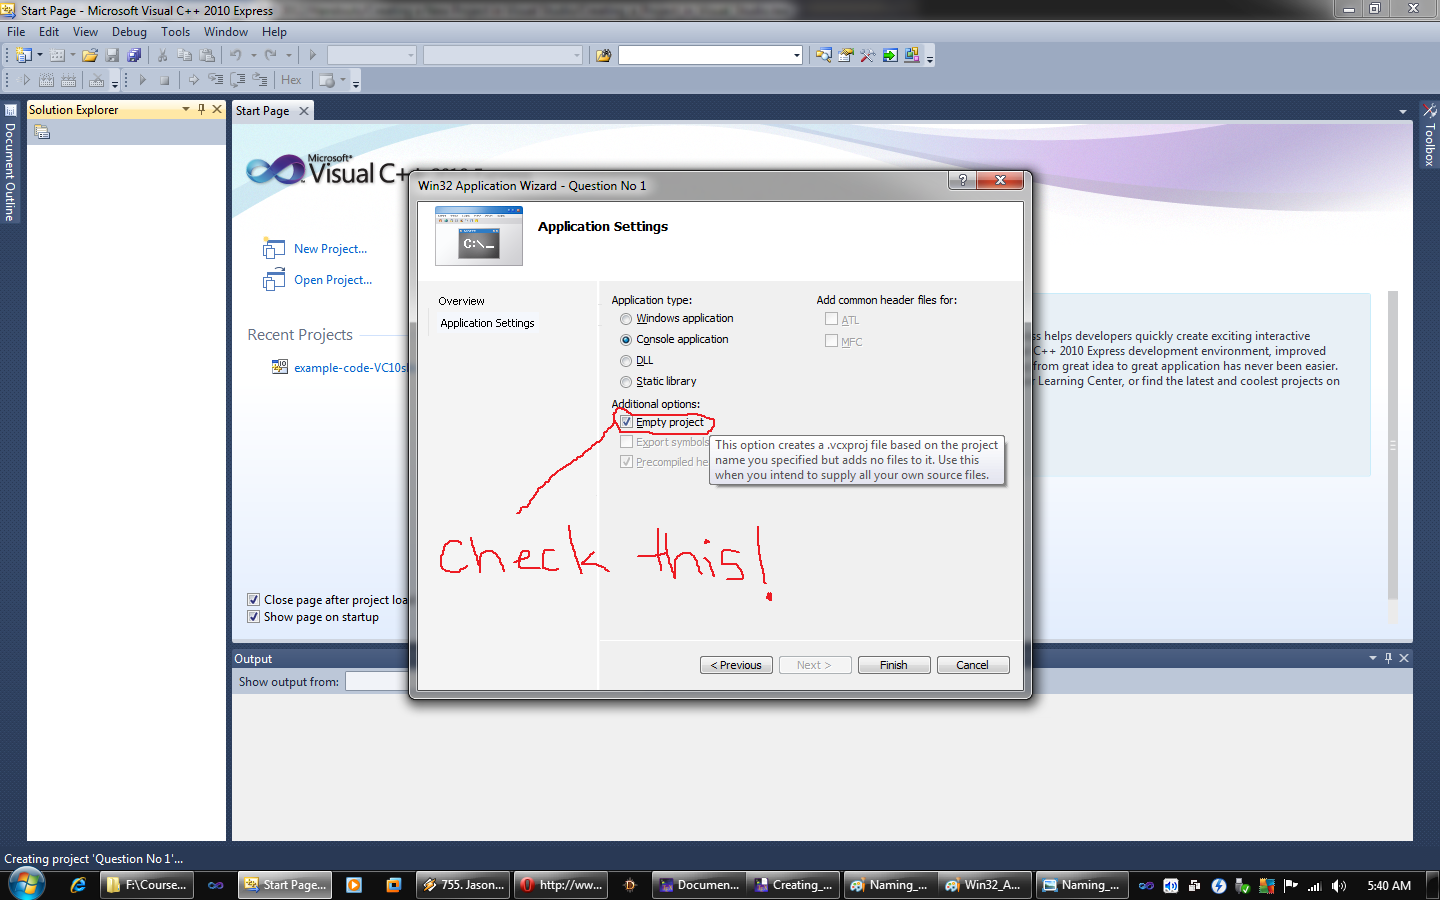
\includegraphics[width=\textwidth]{Application_Settings_Empty_Project.png}
\caption{Creating an empty project}
\end{figure}

\section{Building/Compiling and Running Your Program}

\subsection{Solution Explorer}
After creating your solution/project make sure that \verb|Solution Explorer| is visible. If it is hidden, enable it by navigating to \verb|View > Other Windows > Solution Explorer|\footnotemark~or with the short-cut key \verb|Ctrl+Alt+L|. Solution Explorer gives an overview of your solution. You can view all the projects and code files contained in your solution space and navigate between different files and projects.

\footnotetext[1]{The instructions may vary depending on the layout of Visual Studio. By default Visual C++ 2010 Express Edition has \textit{Basic Layout}. You can change that to \textit{Expert Layout} by navigating to \texttt{Tools > Settings > Expert Settings}.}
\begin{figure}[H]
\centering
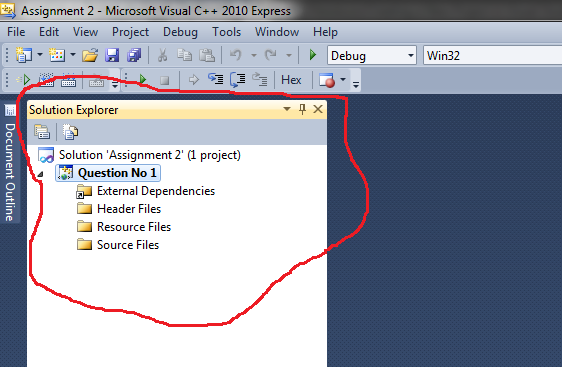
\includegraphics[scale=0.5]{Solution_Explorer.png}
\caption{The Solution Explorer Window}
\end{figure}

\subsection{Adding Files to Project}
Before you start writing your code you need to add the .cpp source file to your project. Right-click the \verb|Source Files| folder from Solution Explorer and \verb|Add| a \verb|New Item|. A new dialog box will appear. Make sure you select \verb|C++ File (.cpp)| from the list of items. Name your file and click \verb|Add|.
\begin{figure}[H]
\centering
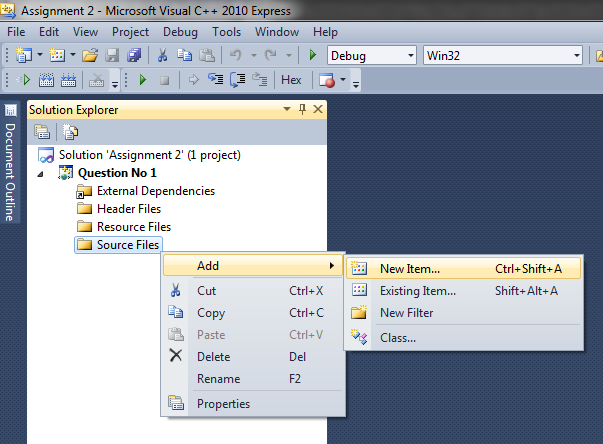
\includegraphics[scale=0.6]{Add_New_Item.png}
\caption{Adding new items to project}
\end{figure}
\begin{figure}[H]
\centering
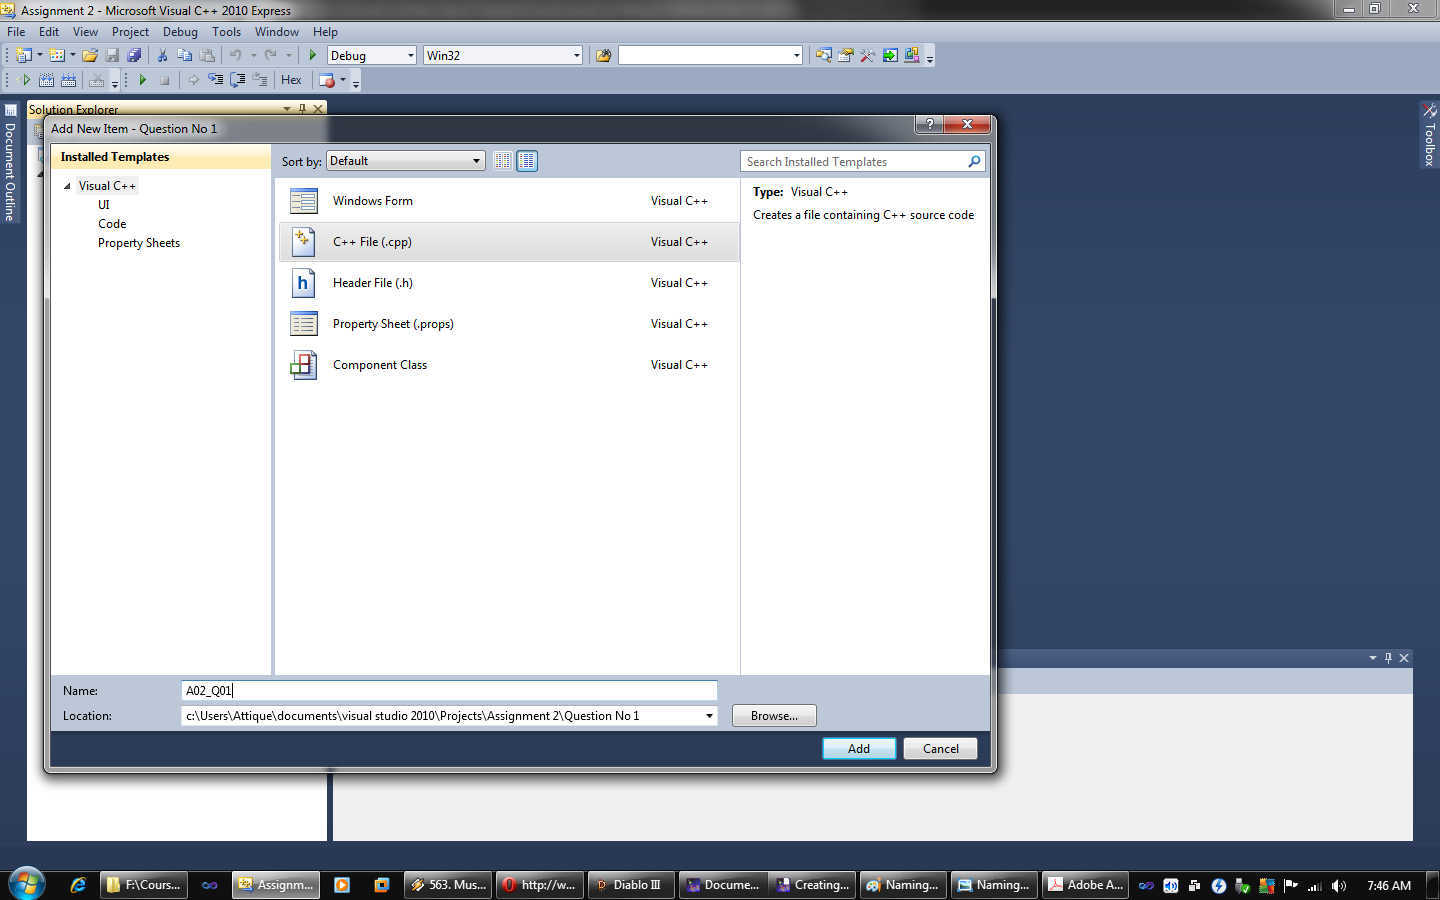
\includegraphics[width=\textwidth]{Add_New_Item_Dialog.png}
\caption{Adding a C++ File (.cpp)}
\end{figure}

\subsection{Navigating Through Errors}
The solution can be built (compiled) using the \verb|F7|. If build is successful, you will get the appropriate message in the output window. Otherwise, a description of all errors will be displayed in \verb|Output| window. You can navigate through error and warning messages with \verb|F4| key. A convenient way to navigate errors is to use the \verb|Error List|. You can bring it up by \verb|View > Other Windows > Error List|.
\begin{figure}[H]
\centering
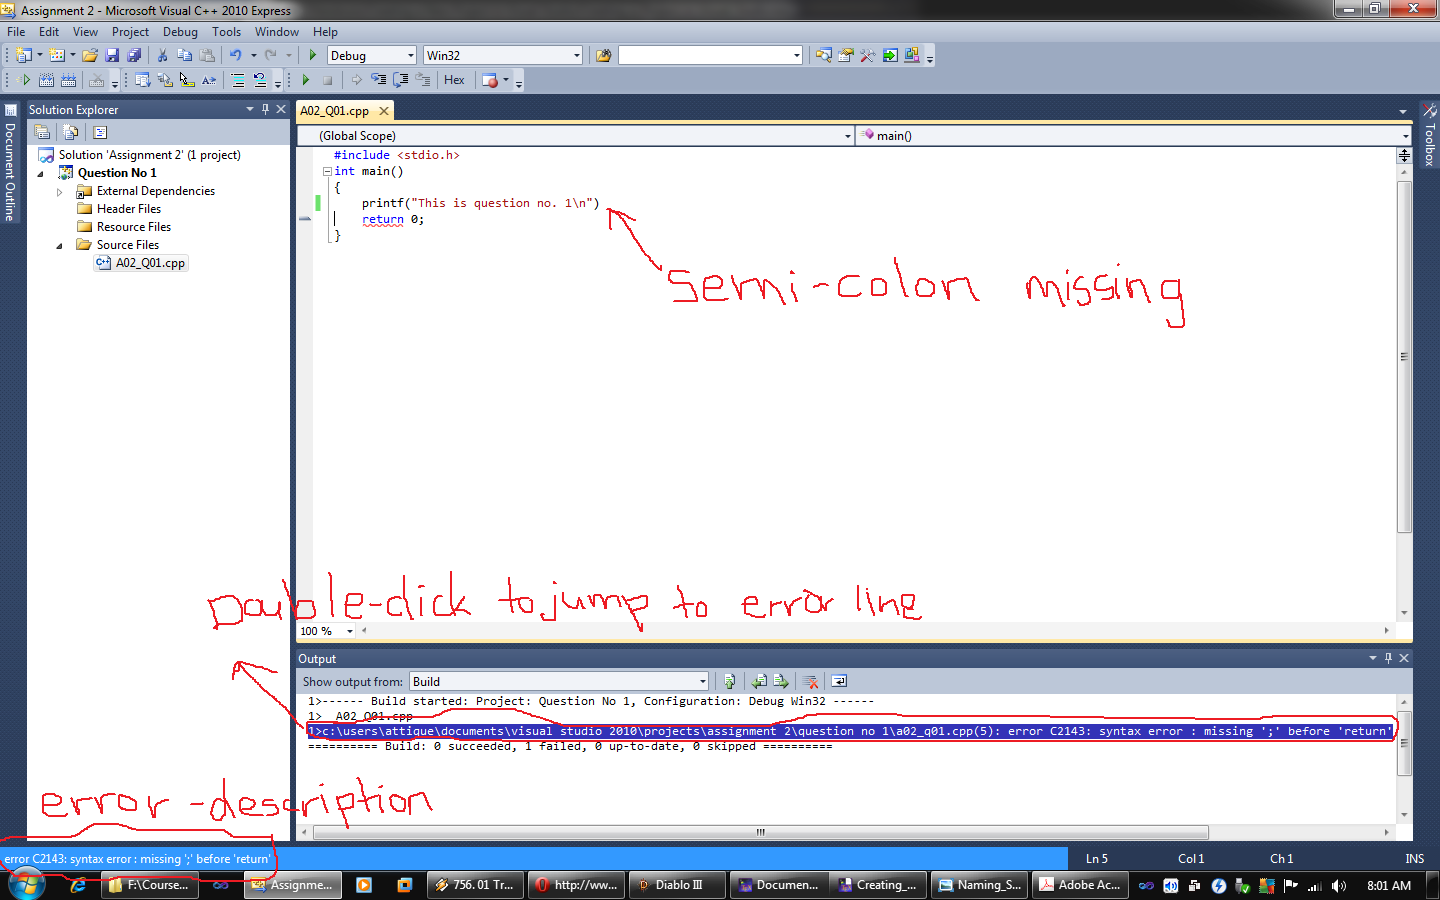
\includegraphics[width=\textwidth]{Compilation_Error.png}
\caption{Error(s) during build}
\end{figure}
\begin{figure}[H]
\centering
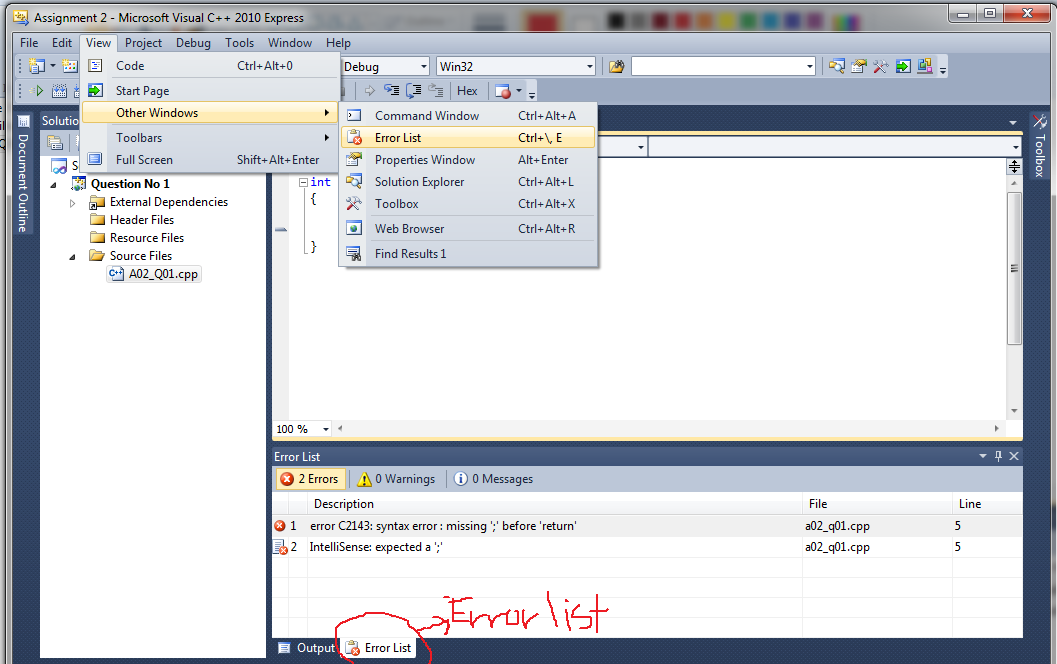
\includegraphics[scale=0.4]{Error_List.png}
\caption{Displaying the Error List}
\end{figure}

\subsection{Program Execution and Debugging}
After a successful \verb|Build| you can test your program by either running the executable\\ (\verb|Start without Debugging, Ctrl+F5|) or start debugger (\verb|F5|). Debugger will stop only at any \verb|Breakpoints| in the program and will exit if there aren't any breakpoints or no input directives. To single-step through your program in debug mode use the \verb|Step Over| key (\verb|F10|). Breakpoints can be placed by moving the cursor to desired line in your code and pressing the \verb|F9| key. Pressing \verb|F9| again will remove an already existing breakpoint.
\begin{figure}[H]
\centering
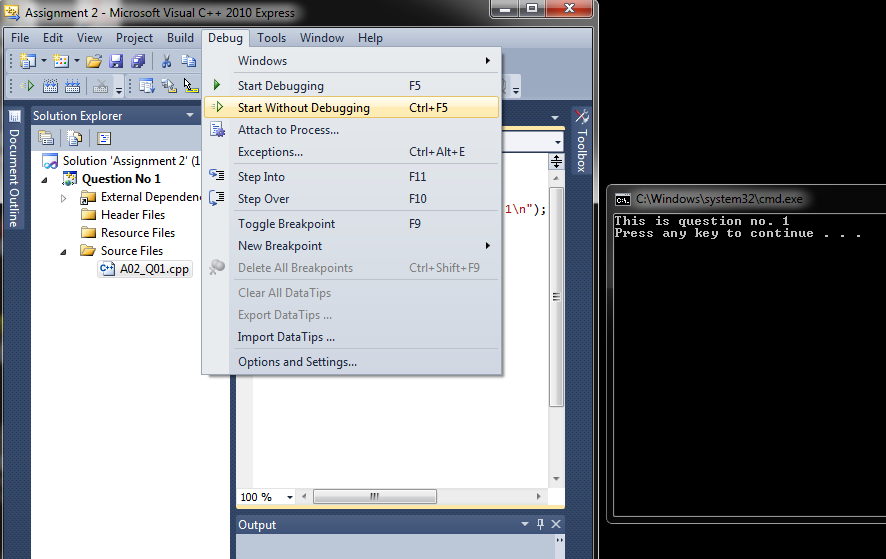
\includegraphics[scale=0.5]{Start_Without_Debugging.png}
\caption{Program execution}
\end{figure}

\section{Adding New Projects to an Existing Solution}
We're now going to add a new project to our solution and name it \verb|Question No 2|. In the Solution Explorer window right-click on solution name and add a new project. Follow the steps from Section 2 for creating a new empty project of type \verb|Win32 Consolte Application|.
\begin{figure}[H]
\centering
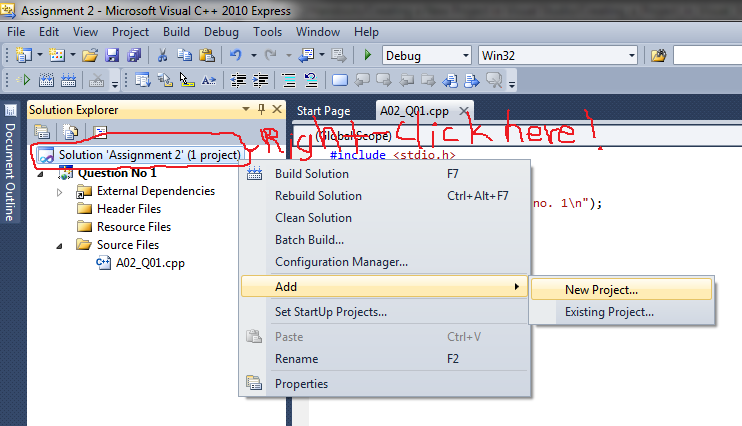
\includegraphics[scale=0.6]{Add_New_Project.png}
\caption{Adding new projects to solution}
\end{figure}

Add a C++ source file (.cpp) to your project following the steps in Section 3.2. We'll name our file \verb|A02_Q02.cpp| here. Before you can compile and run your new project you must set it as \verb|Active Project|. This can be done by right-clicking the project name (Question No 2 in this case) and selecting\\ \verb|Set as StartUp Project| from the drop down menu. Active project name will be in \textbf{bold}. Figure 14 shows the complete solution space with output window and \verb|Question No 2| selected as active project.
\begin{figure}[H]
\centering
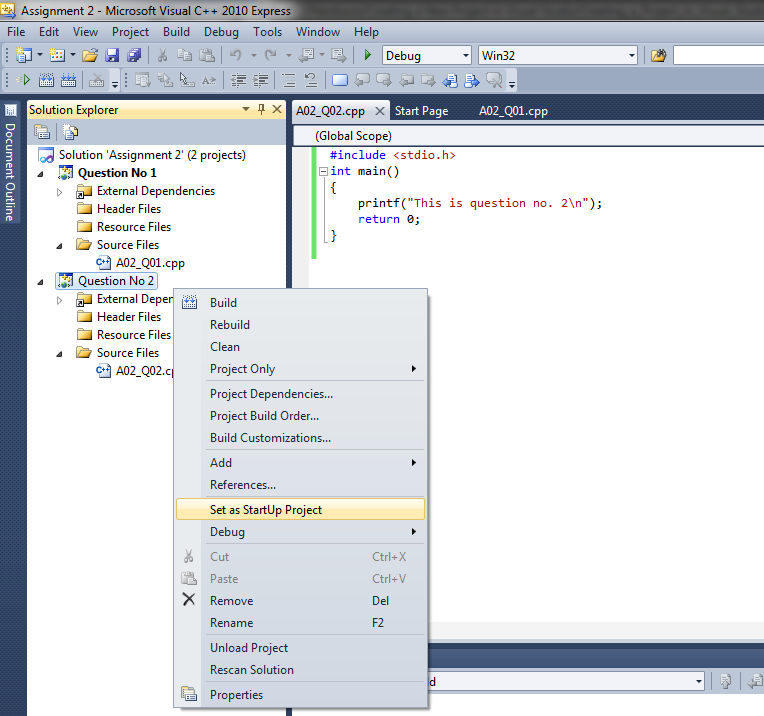
\includegraphics[scale=0.6]{Setting_Active_Project.png}
\caption{Setting active project}
\end{figure}

\section{Transferring Solutions}
In order to transfer your work you need to copy the whole solution folder located in the \verb|My Documents| folder. The solution folder contains a \verb|[Solution Name].sln| file. You can open your solution by double-clicking on this file, provided that Visual Studio is installed on that particular computer.

The solution folder also contains separate folders for each project in the solution. The C++ code (.cpp) files are located in their respective project folders. In order to conserve space you can delete any folders named \verb|Debug| in the solution or project folders. You can also delete \verb|ipch| folders or any \verb|.sdf| files. The \verb|Debug| folder in solution folder contains executables from each project.

\begin{figure}[H]
\centering
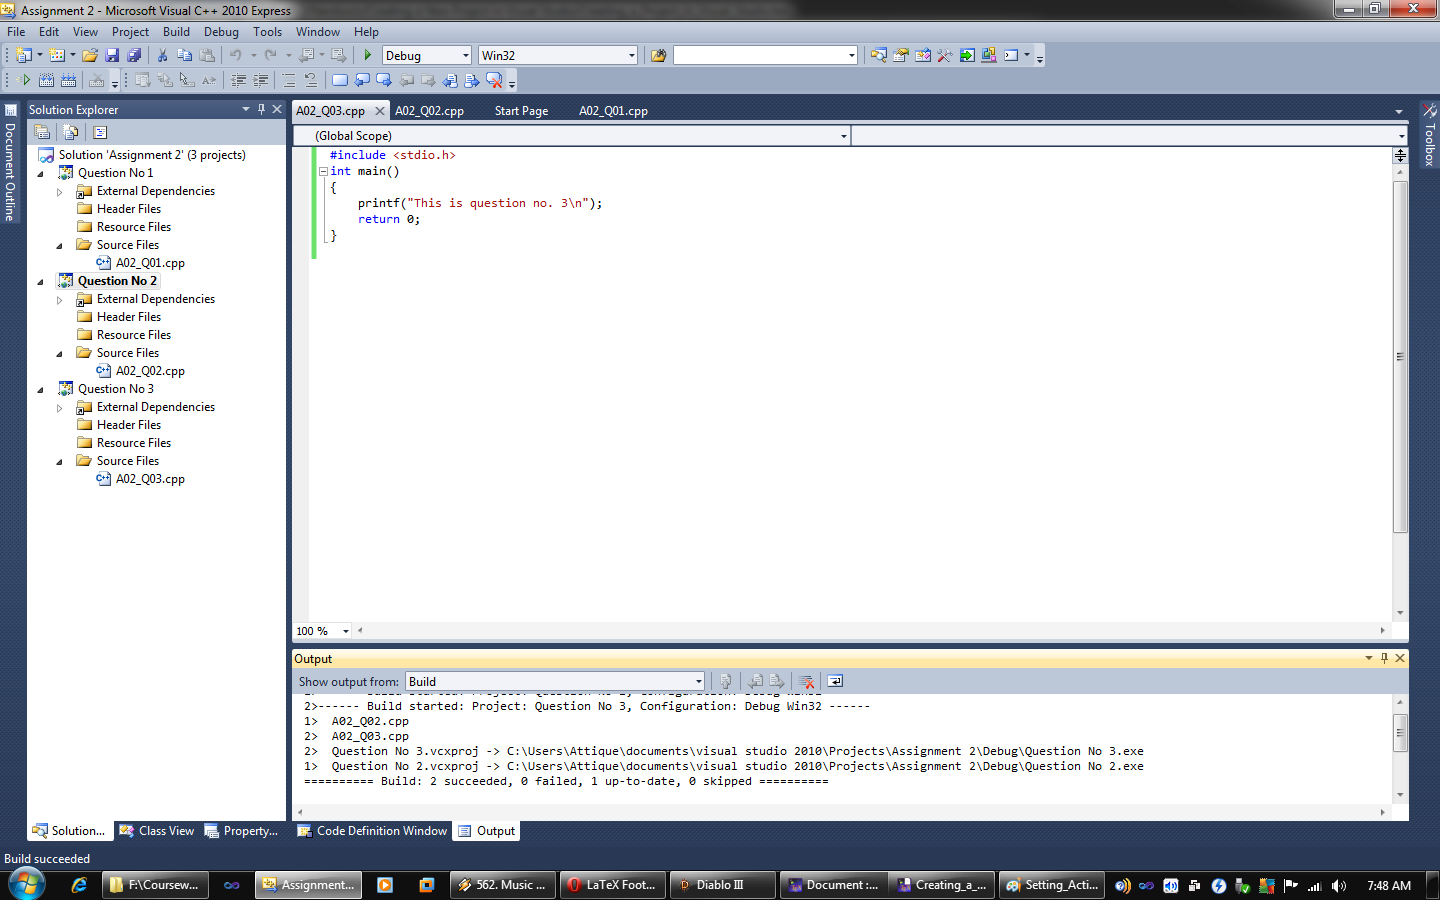
\includegraphics[width=\textwidth]{Final_Solution_Space.png}
\caption{Final solution space}
\end{figure}

\begin{figure}[H]
\centering
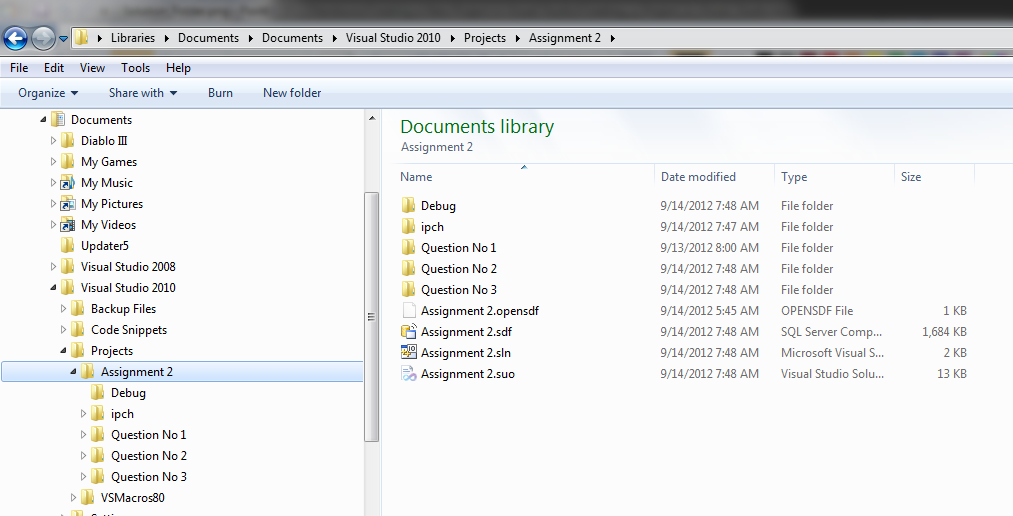
\includegraphics[width=\textwidth]{Solution_Folder.png}
\caption{Solution folder}
\end{figure}
\end{document}



\end{document}